\documentclass[border=10pt]{standalone}
\usepackage[svgnames]{xcolor}
\usepackage{amsmath}
\usepackage{pgfplots}
\pgfplotsset{compat=newest}
\usepackage[sfdefault]{FiraSans}
\usepackage{FiraMono}
\renewcommand*\familydefault{\sfdefault}
\begin{document}
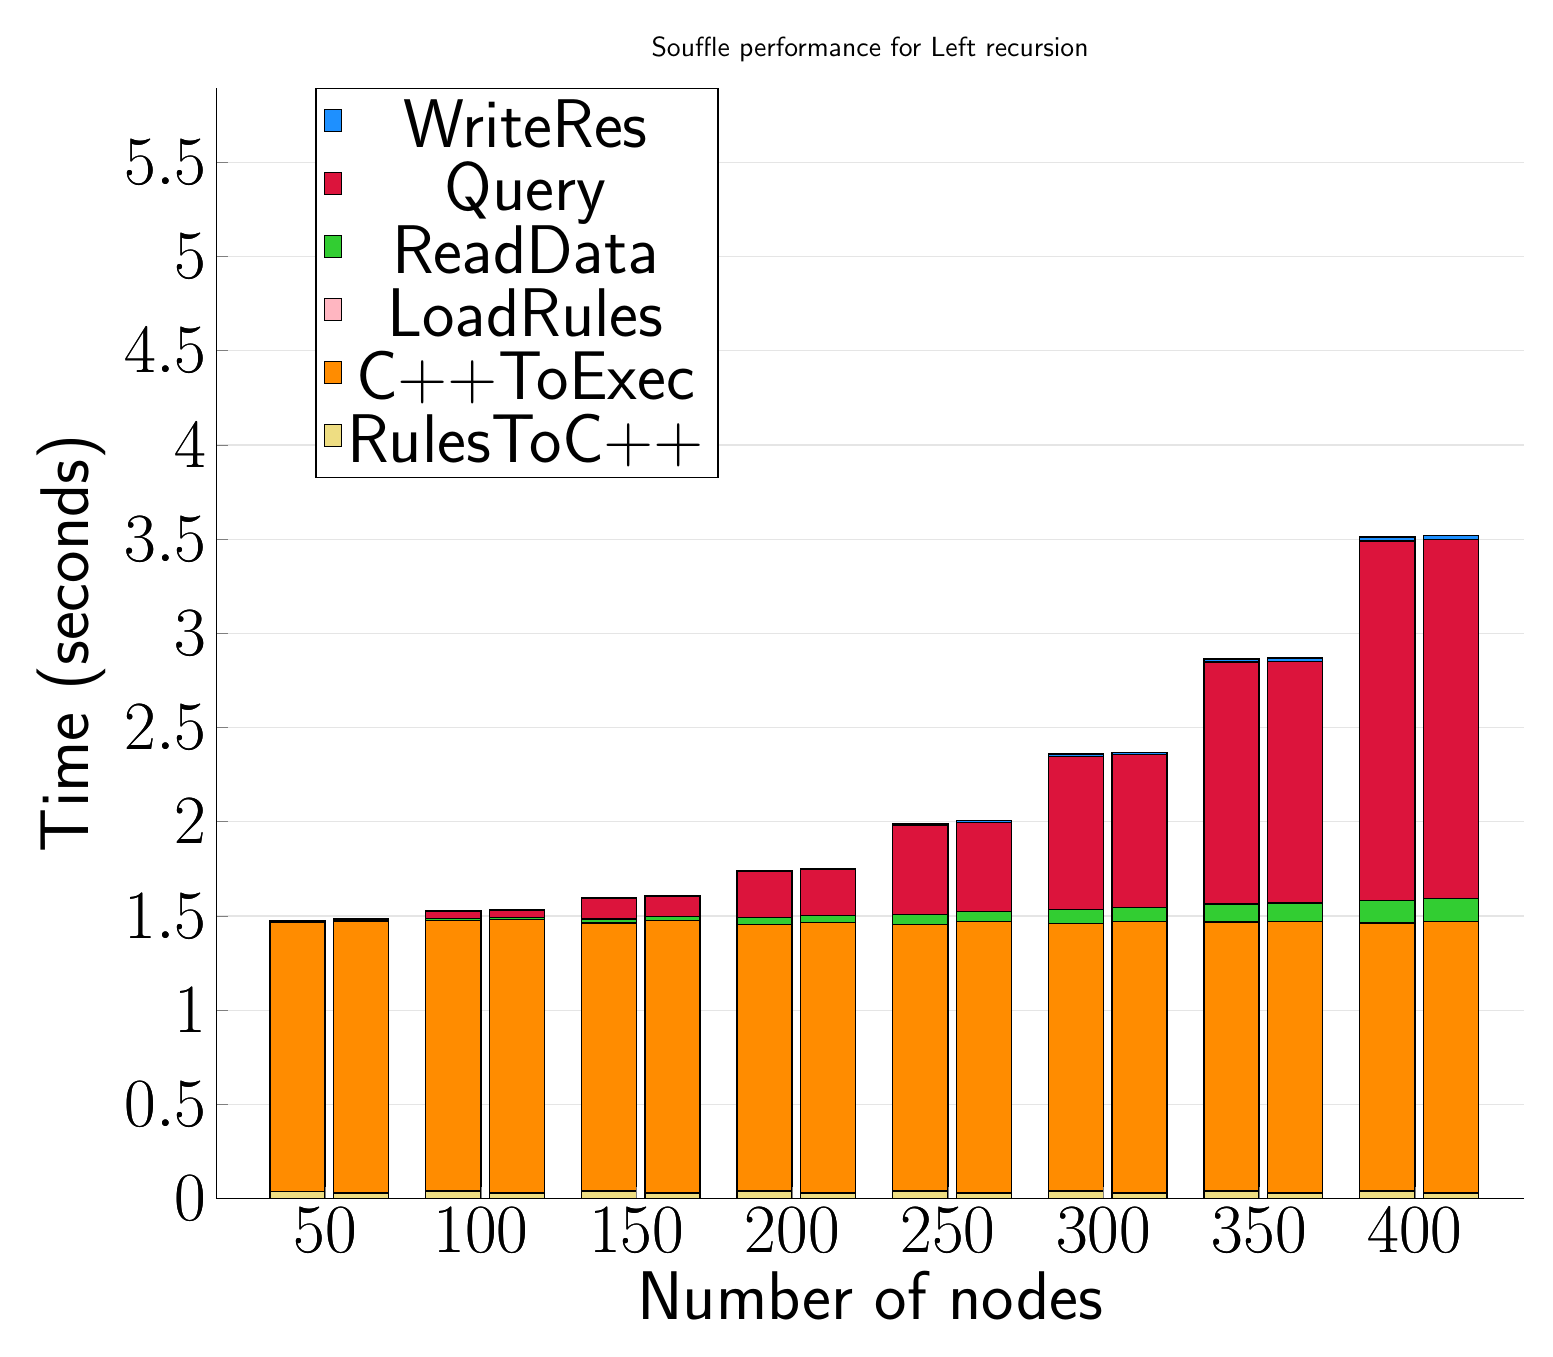
\begin{tikzpicture}
\begin{axis}[
   ybar stacked,
   title={Souffle performance for Left recursion},
   bar shift=-10pt,
   width=1.5\textwidth,
   bar width=0.7cm,
   ymajorgrids, tick align=inside,
   major grid style={draw=gray!20},
   xtick=data,
   ymin=0, ymax=5.895328,
   axis x line*=bottom,
   axis y line*=left,
   enlarge x limits=0.1,
   legend style={
       at={(0.23, 1)},
       anchor=north,
       legend columns=1,
       font=\Huge,
   },
   ylabel={Time (seconds)},
   xlabel={Number of nodes},
   label style={font=\Huge},
   tick label style={font=\Huge},
]
\addlegendimage{fill=DodgerBlue, draw=black, line width=0.2pt}
\addlegendentry{WriteRes}
\addlegendimage{fill=Crimson, draw=black, line width=0.2pt}
\addlegendentry{Query}
\addlegendimage{fill=LimeGreen, draw=black, line width=0.2pt}
\addlegendentry{ReadData}
\addlegendimage{fill=LightPink, draw=black, line width=0.2pt}
\addlegendentry{LoadRules}
\addlegendimage{fill=DarkOrange, draw=black, line width=0.2pt}
\addlegendentry{C++ToExec}
\addlegendimage{fill=LightGoldenrod, draw=black, line width=0.2pt}
\addlegendentry{RulesToC++}
\addplot +[fill=LightGoldenrod, draw=black, line width=0.5pt] coordinates {
    (50, 0.03899998664855957)
    (100, 0.04000000953674317)
    (150, 0.039999985694885255)
    (200, 0.04000000953674317)
    (250, 0.04000000953674317)
    (300, 0.039999961853027344)
    (350, 0.040999960899353025)
    (400, 0.039999985694885255)
};
\addplot +[fill=DarkOrange, draw=black, line width=0.5pt] coordinates {
    (50, 1.425000047683716)
    (100, 1.4359999895095825)
    (150, 1.4219999074935914)
    (200, 1.4140000104904176)
    (250, 1.4149999856948852)
    (300, 1.4200000762939453)
    (350, 1.4260000705718994)
    (400, 1.422000002861023)
};
\addplot +[fill=LightPink, draw=black, line width=0.5pt] coordinates {
    (50, 0.0001230793)
    (100, 8.414169999999999e-05)
    (150, 0.0001086208)
    (200, 0.0001223086)
    (250, 0.00011189159999999999)
    (300, 0.00012099999999999999)
    (350, 0.00011904159999999999)
    (400, 8.52251e-05)
};
\addplot +[fill=LimeGreen, draw=black, line width=0.5pt] coordinates {
    (50, 0.0028740170000000004)
    (100, 0.009753862000000002)
    (150, 0.02148211)
    (200, 0.03701945)
    (250, 0.05347518999999999)
    (300, 0.0742822)
    (350, 0.09662812)
    (400, 0.12050659999999999)
};
\addplot +[fill=Crimson, draw=black, line width=0.5pt] coordinates {
    (50, 0.006885354000000001)
    (100, 0.0383157)
    (150, 0.1084532)
    (200, 0.2455677)
    (250, 0.4737724)
    (300, 0.812308)
    (350, 1.283789)
    (400, 1.907538)
};
\addplot +[fill=DodgerBlue, draw=black, line width=0.5pt] coordinates {
    (50, 0.0007056666000000001)
    (100, 0.0016780369999999998)
    (150, 0.003566896)
    (200, 0.00597848)
    (250, 0.008742616)
    (300, 0.01270464)
    (350, 0.01698633)
    (400, 0.02230191)
};
\end{axis}
\begin{axis}[
   ybar stacked,
   bar shift=13pt,
   width=1.5\textwidth,
   bar width=0.7cm,
   ymajorgrids, tick align=inside,
   major grid style={draw=none},
   xtick=data,
   ymin=0, ymax=5.895328,
   axis x line*=none,
   axis y line*=none,
   enlarge x limits=0.1,
   label style={font=\Huge},
   tick label style={font=\Huge},
]
\addplot +[fill=LightGoldenrod, draw=black, line width=0.5pt] coordinates {
    (50, 0.030000000000000006)
    (100, 0.030000000000000006)
    (150, 0.030000000000000006)
    (200, 0.030000000000000006)
    (250, 0.030000000000000006)
    (300, 0.030000000000000006)
    (350, 0.030000000000000006)
    (400, 0.030000000000000006)
};
\addplot +[fill=DarkOrange, draw=black, line width=0.5pt] coordinates {
    (50, 1.4439999999999997)
    (100, 1.452)
    (150, 1.4459999999999997)
    (200, 1.4349999999999998)
    (250, 1.4399999999999997)
    (300, 1.44)
    (350, 1.4419999999999997)
    (400, 1.4409999999999996)
};
\addplot +[fill=LightPink, draw=black, line width=0.5pt] coordinates {
    (50, 0.0001222)
    (100, 8.36e-05)
    (150, 0.00010760000000000001)
    (200, 0.00012130000000000001)
    (250, 0.00011119999999999999)
    (300, 0.00012050000000000002)
    (350, 0.00011789999999999999)
    (400, 8.47e-05)
};
\addplot +[fill=LimeGreen, draw=black, line width=0.5pt] coordinates {
    (50, 0.0028732000000000002)
    (100, 0.009751099999999997)
    (150, 0.0214779)
    (200, 0.03701229999999999)
    (250, 0.053462300000000004)
    (300, 0.07427120000000001)
    (350, 0.0966102)
    (400, 0.1204414)
};
\addplot +[fill=Crimson, draw=black, line width=0.5pt] coordinates {
    (50, 0.006883200000000001)
    (100, 0.038270000000000005)
    (150, 0.10828600000000002)
    (200, 0.2454057)
    (250, 0.47343029999999997)
    (300, 0.8119078999999999)
    (350, 1.2833649999999999)
    (400, 1.9063639999999995)
};
\addplot +[fill=DodgerBlue, draw=black, line width=0.5pt] coordinates {
    (50, 0.0007049999999999999)
    (100, 0.0015942)
    (150, 0.0032892)
    (200, 0.0056758)
    (250, 0.008724699999999998)
    (300, 0.012534299999999998)
    (350, 0.0169392)
    (400, 0.0222286)
};
\end{axis}
\end{tikzpicture}

\end{document}
